%!TEX root=../document.tex

\section{How did it all start?}

Countries around the European Union have not been ideal places to live recently. The countries, that are included in this crisis, are mostly from the Mideast and Africa. All together nine civil wars are going on in these regions. This is why there are so many refugees fleeing for their lives. About 11 million people of the population of Syria have been forced to leave their homes, with over four million refugees from other countries.

Syria has been going through a brutal civil war for four years now. In 2011, Syria many government protests broke out.
Back then the current president with the name ''Bashar al-Assad'' did not appreciate these and responded with a massive killing spree, killing those who disagreed with him. This prompted resistors to build groups, and arm them with lethal weapons against him. This developed into a full-blown civil war, with at least a thousand of rebel groups with different mindsets.

Civil wars are not the only reason for this crisis. Weak economies causing the population to leave their places and find better ones, with more stable political and social environment. And if that is not enough, an organisation called ISIS (Islamic State of Iraq and Syria) developed through this time. They use the downsides of these developing countries for their advantage. Recruiting young people to fight on their side for their ideology.

\begin{figure}[!h]
	\begin{center}
		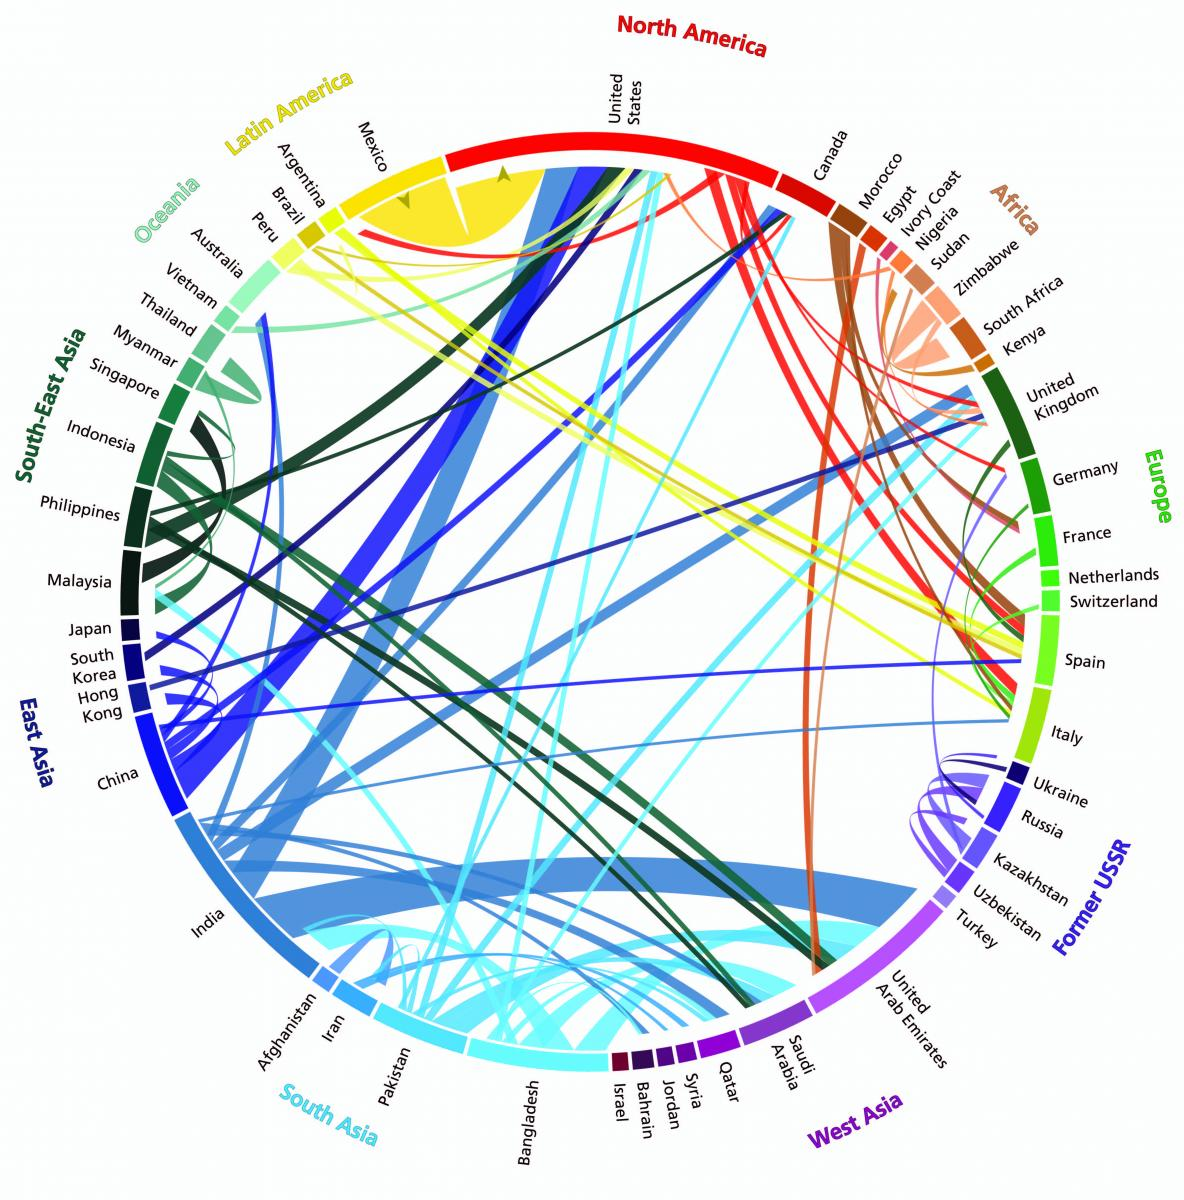
\includegraphics[width=0.68\linewidth]{images/refugee_map}
		\caption{Global refugee network map}
	\end{center}
\end{figure}

\newpage
\section{Civil wars}

\subsection{Iran - PJAK conflict}
The Iran-PJAK (Kurdistan Free Life Party) conflict is an armed conflict between the Islamic Republic or Iran and the ethnic secessionist Kurdisch guerrilla group PJAK, which began back in 2004. The group had been carrying out attacks in the Kurdistan Province of Iran and other Kurdish-inhabited areas. Following large clashes in summer 2011, a cease-fire was declared between the parties, with Iran claiming victory and PJAK ending all armed operations as of 29 September 2011. Since then, several violent incidents have occurred.

\begin{itemize}
	\item \textbf{Iran}
		\subitem supported by \textbf{Turkey}
	\item \textbf{Kurdistan Free Life Party (PJAK)}
\end{itemize}

Since the Iranian Revolution, there has been an ongoing conflict between Iran’s central government and Kurdish political movements rooted in the predominantly Kurdish region of western Iran. The level of violence has ebbed and flowed with peaks of serious conflict in 1979, the early eighties and the early nineties.

Kurdish casualties are estimated by the Kurdish Democratic Party of Iran (KDPI) at more than 30,000 civilian dead in addition to 4,000 Kurdish fighters. Along with the dead, there have been tens of thousands of people imprisoned, hundreds of villages destroyed and hundreds of thousands of people displaced. The local economy of an already under-developed region has been severely damaged by the conflict, as of course has the Iranian economy as a whole.

According to founding members of PJAK, however, the group began in Iran around 1997 as an entirely peaceful student-based human rights movement. The group was inspired by the success of Iraq's Kurdish autonomous region. Discouraged by the failure of previous Kurdish revolts, however, PJAK's leaders initially worked only to maintain and build a Kurdish national identity and to thwart the Iranian government's attempts to re-brand Iranian Kurds as ethnic Persians or Aryans.
PJAK transformed from a civil rights movement to a more ambitious and multi-directional independence movement.
\newpage



\begin{figure}[!h]
	\begin{center}
		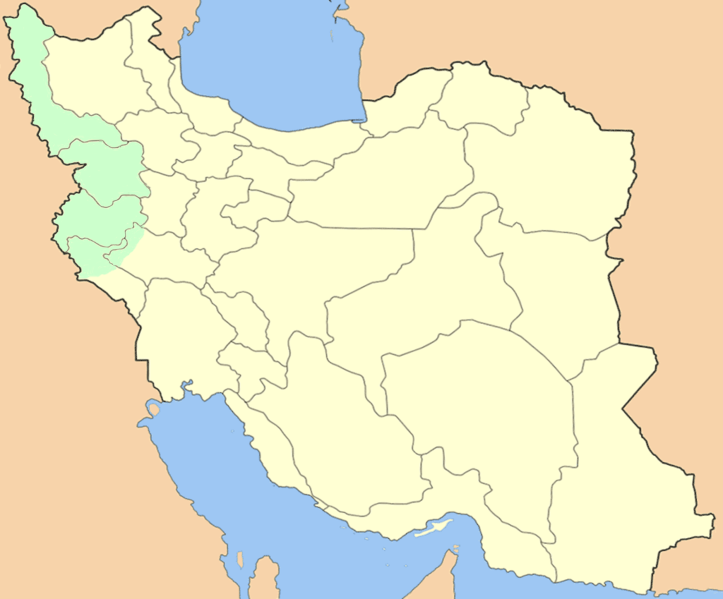
\includegraphics[width=0.5\linewidth]{images/Map_of_Iranian_Kurdistan}
		\caption{Map of Iranian Kurdistan}
	\end{center}
\end{figure}

It is clear to see the green marked area on the map, this is the epicenter of PJAK insurrection.
Following regions are included:
\begin{itemize}
	\item West-Azerbaijan
	\item Kordestan
	\item Kermanshah Provinces in Iran
	\item Kurdistan Region
\end{itemize}

There are not many reports or data to rely on, because every party involved in this civil war, accused others instead of taking fault on themselve. \textbf{So summed up following facts clearly point out:}

\begin{itemize}
	\item Iran vs Kurdistan Free Party (PJAK)
	\item around 34,000 casualties
	\item PJAK build on a national identity
	\item War Zone - West area of Iran
	\item Facts are not proven completely
\end{itemize}

\subsection{Syria Civil War}
Syria has been going through a brutal civil war for four years now. In 2011, Syria many government protests broke out.
Back then the current president with the name ''Bashar al-Assad'' did not appreciate these and responded with a massive killing spree, killing those who disagreed with him. This prompted resistors to build groups, and arm them with lethal weapons against him. This developed into a full-blown civil war, with at least a thousand of rebel groups with different mindsets.

Both sides leaked information, about having chemical weapons in their property. In August 2013, images surfaced that appeared to show a massive chemical attack on civilians in Syria. The United States blamed Assad and Assad blamed the rebels.
For a time it looked like the US was on the brink of military intervention in Syria. Then the UN (United Nations) and Assad cut a deal, to destroy all chemical weapons. The talk of intervention cooled off, for a while. \newline


\textbf{Main belligerents: }
\begin{itemize}
	\item \textbf{Syrian Goverment (NPF)}
		\subitem supported by Russia
	\item \textbf{Opposition}
		\subitem supported by United States
	\item \textbf{ISIL (ISIS)}
	\item \textbf{Army of Conquest}
	\item \textbf{Rojava (SDC)}
	\item \textbf{Combined Joint Task Force}
		\subitem US, States of Europe, Turkey, Saudi Arabia
\end{itemize}

\newpage

\begin{figure}[!h]
	\begin{center}
		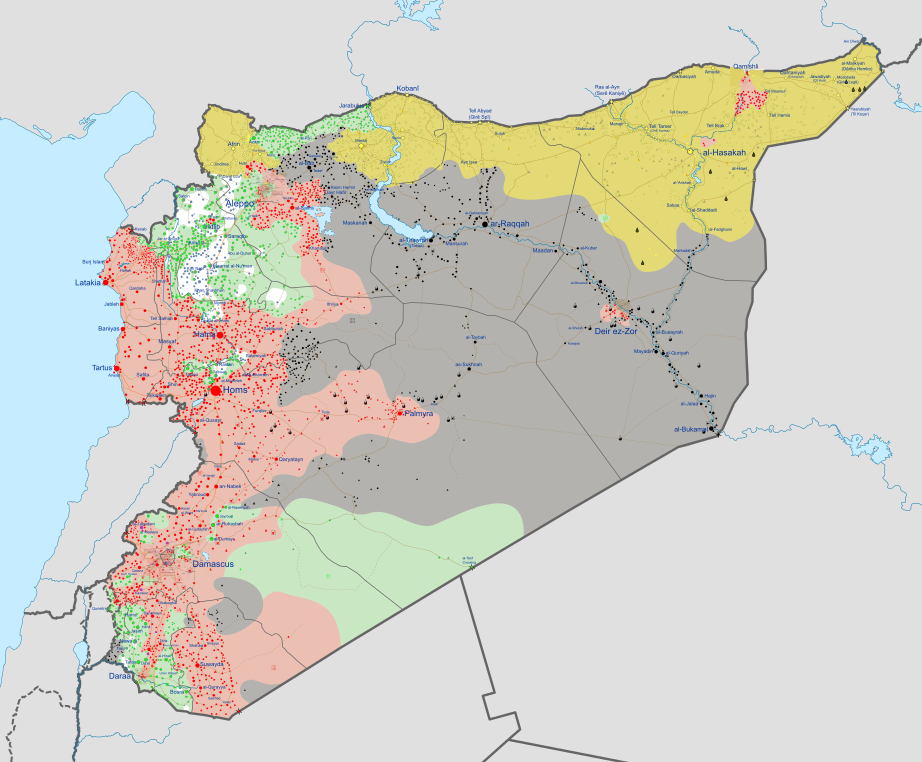
\includegraphics[width=\linewidth]{images/Syrian_Civil_War_map}
		\caption{Syrian civil war map}
	\end{center}
\end{figure}

\textbf{current military situation:}\newline
\textit{Red}: \textbf{Syrian Goverment}
\textit{Green}: \textbf{Syrian Oppostition}
\textit{Yellow}: \textbf{Federation of North Syria (SDF)}
\textit{Grey}: \textbf{Islamic State of Iraq and the Levant}
\textit{White}: \textbf{Jabhat Fateh al-Sham}

\newpage

At the start of the war, discontent against the government was said to be the strongest in Syria's poor areas, predominantly among conservative Sunnis. These included cities with high poverty rates, such as Daraa and Homs and the poorer districts of large cities.

Socioeconomic inequality increased significantly after free market policies were initiated by Hafez al-Assad in his later years, and accelerated after Bashar al-Assad came to power. With an emphasis on the service sector, these policies benefited a minority of the nation's population, mostly people who had connections with the government, and members of the Sunni merchant class of Damascus and Aleppo. The country also faced particularly high youth unemployment rates.

This coincided with the most intense drought ever recorded in Syria. It lasted from 2007 to 2010 and resulted in widespread crop failure, an increase in food prices and a mass migration of farming families to urban centers. Syria had also received in the same period around 1.5 million refugees from Iraq.

By 2011, Syria was facing steep rises in the prices of commodities and a clear deterioration in the national standard of living.

\textbf{So summed up following facts clearly point out:}
\begin{itemize}
	\item Al-Assad vs. Rebels vs. World
	\item origin of modern refugee crisis
	\item chemical weapons
	\item thousands of rebel-groups with different mindsets
	\item human rights
\end{itemize}



\section{USA vs. Russia, War for resources}
The Syrian war often seems like a big confusing mess but one factor that is not often mentioned could be the key to unlocking the conflict.
Many have questioned why Russia became involved in the Syrian war but often overlook the fight over natural gas.
Russia currently supplies Europe with a quarter of the gas it uses for heating, cooking, fuel and other activities.
In fact 80 per cent of the gas that Russian state-controlled company Gazprom produces is sold to Europe, so maintaining this crucial market is very important.
But Europe does not like being so reliant on Russia for fuel and has been trying to reduce its dependence. It’s a move that is supported by the United States as it would weaken Russian influence over Europe.
This has not gone down well with Russia, which uses its power over gas as political leverage and has a history of cutting off supply to countries during conflicts. It has even gone to war in Georgia and Ukraine to disrupt plans to export gas from other parts of the Middle East.
Russia has always used gas as an instrument of influence. The more you owe Gazprom, the more they think they can turn the screws.Much of Russia’s power comes from established pipelines used to transport gas to Europe cheaply. But other countries are now trying to get around Russia and provide new sources of gas to Europe.
In 2015 US President Barack Obama spoke openly about the need for Europe to reduce its reliance on Russian gas following the conflict in Ukraine.
The US also wants to use its own natural gas supply, recently developed through fracking, to undercut Russian supply. But it will be years before the US will be in a position to ship this overseas.
The US is not the only country trying to outmanoeuvre Russia, and this is where the role of Syria becomes more important.

\textbf{Two new pipelines} \newline
Before the civil war, two competing pipelines put forward by Qatar and Iran aimed to transport gas to Europe through Syria.
Qatar’s plans were first put forward in 2009 and involved building a pipeline from the Persian Gulf via Saudi Arabia, Jordan, Syria and Turkey.
The gas field located 3000 metres below the floor of the Persian Gulf is the largest natural gas field in the world. Qatar owns about two-thirds of the resource but can’t capitalise on it fully because it relies on tankers to deliver it to other countries and this makes its gas more expensive than Russia’s.
It was hoped the pipeline would provide cheaper access to Europe but Syrian President Bashar al Assad refused to give permission for the pipeline to go through his territory. Some believe Russia pressured him to reject the pipeline to safeguard its own business.


\begin{figure}[!h]
	\begin{center}
		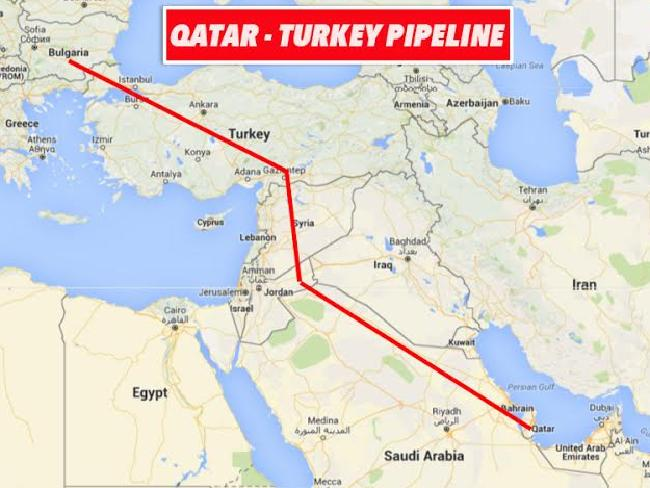
\includegraphics[width=0.5\linewidth]{images/pipe_line_turkey}
		\caption{The proposed gas pipeline from Qatar via Saudi Arabia, Jordan, Syria and Turkey to Europe.}
	\end{center}
\end{figure}

\newpage
In the meantime Iran, which owns the other smaller, share of the Persian Gulf gas field, decided to lodge its own rival plan for a \$10 billion pipeline to Europe via Iraq and Syria and then under the Mediterranean Sea.

\begin{figure}[!h]
	\begin{center}
		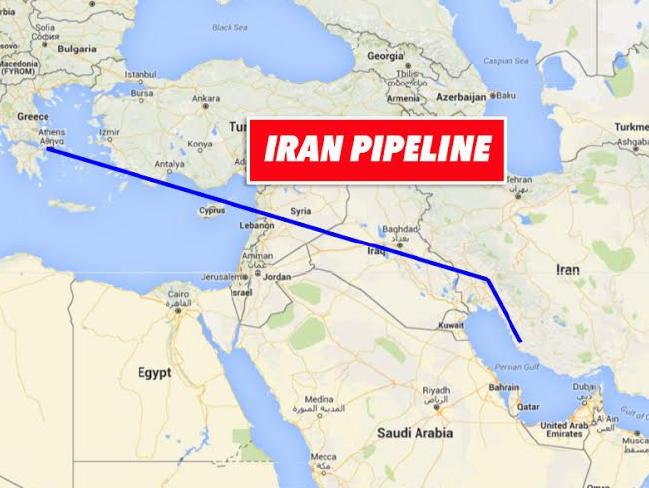
\includegraphics[width=0.5\linewidth]{images/pipe_line_iran}
		\caption{Pipeline from Iran via Iraq and Syria to Europe.}
	\end{center}
\end{figure}

These plans apparently had Russia’s blessing, possibly because it could exert more influence over Iran, which, unlike Qatar, did not host a US air base.
Assad signed off on the Iran plan in 2012 and it was due to be completed in 2016 but it was ultimately delayed because of the Arab Spring and the civil war.
Many countries supporting or opposing the war against Assad have links to these pipeline plans.
Failed pipeline bidder Qatar is believed to have funded anti-Assad rebel groups by \$3 billion between 2011 and 2013. Saudi Arabia has also been accused of funding the terrorist group.
In contrast Orenstein and Romer noted the successful pipeline bidder, Iran, was believed to be helping Assad by running the Syrian army, supplying it with weapons and even troops.

Viewed through a geopolitical and economic lens, the conflict in Syria is not a civil war, but the result of larger international players positioning themselves on the geopolitical chessboard in preparation for the opening of the pipeline.
Just as the 2003 Iraq War has been linked to oil in the Persian Gulf, Syria may turn out to be all about gas.\newline

\textbf{So summed up following facts clearly point out:}
\begin{itemize}
	\item Europe´s gas resource relies on Russia
	\item United Stats try to weak influence of Russia over Europe
	\item Other countries try to get around Russia to provide new sources for Europe
	\item Two new pipelines
	\item Qatar-Turkey pipeline
	\item Iran pipeline
	\item viewed through a geopolitical lens, conflict in Syria is not a civil war
	
\end{itemize}


\section{Islamic State of Iraq and the Levant}

The Islamic State was founded in 2012 during the civil war in Syria. In 2006 the same grouping built however they had no significant power. Through the proclamation of an Islamic State in Iraq and Syria, both organizations combined under the lead of Abu Bakr al Baghdadi. The organization saw itself as competition to al Nusra Front, which is more moderate in the civil war. They recognize other war parties and created strategies against the Syrian government together.

Because of the successes that ISIS could record, many other groups or fighters joined the Islamic State. Local as well as international the ISIS has collected members around the globe, some of them are even in Europe. The international coalition against the Islamic State, led by the United States, could do little tho the organization, since other powers such as Russia, Turkey or Iran have other ideologies. They support the government of Assad, which takes action against militia, which are financed by western countries.

\begin{figure}[!h]
	\begin{center}
		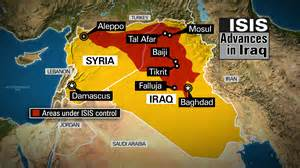
\includegraphics[width=0.5\linewidth]{images/ISIS_area}
		\caption{Area controlled by the Islamic State}
	\end{center}
\end{figure}

But how could the IS become so strong in Iraq? All this is due to the American invasion in Iraq in 2003. At that time sunni milita were heavily fought, because they were supporting the Baath Regime. After the invasion the Iraqi army was disabanded, leaving many of soldiers behind. So these soldiers joined islamic groups.

The state of human rights in territories controlled by the Islamic State of Iraq and the Levant has been criticised by many political, religious and other organizations and individuals. However, ISIS is not alone in committing war crimes in Iraq.  Alarming reports have surfaced about Shiite death squads, some allegedly in Iraqi security force uniforms, operating around Baghdad.  These groups are accused of targeting and killing Sunni civilians.  These executions are reminiscent of the sectarian cleansing that occurred at the height of the United States occupation in 2006 and 2007.  In addition to killings by militia groups, there are also accusations that Iraqi military and police units have massacred Sunni prisoners, some still in their cells.  One news report claims that 69 prisoners were murdered on June 23rd in Hilla.  This is in addition to 52 prisoners that were allegedly executed in Baquba last week.
ISIS’ goal is not only to scare Iraqi Shiites but to provoke them to radicalize, join Iranian-sponsored militias and then commit similar atrocities against Sunnis.  ISIS then hopes to set itself up as the protectors of the Sunni population, helping to consolidate its hold on Sunni population centers.


\textbf{So summed up following facts clearly point out:}
\begin{itemize}
	\item Islamic state founded back in 2012
	\item alliance of rebel groups
	\item controll more than 50\% of Syria
	\item harming Human Rights
	\item executing civilians
	\item global spreaded
\end{itemize}

\section{Historical refugee crisis}

\section{Refugee crisis impact on Europe}

Europe is experiencing one of the most significant influxes of migrants and refugees in its history. Pushed by civil war and terror and pulled by the promise of a better life, huge numbers of people have fled the Middle East and Africa, risking their lives along the way.

More than a million migrants and refugees crossed into Europe in 2015, compared with just 280,000 the year before. The scale of the crisis continues, with more than 135,000 people arriving in the first two months of 2016.

Among the forces driving people to make the dangerous journey are the conflicts in Syria, Iraq and Afghanistan. The vast majority - more than 80ß\% - of those who reached Europe by boat in 2015 came from those three countries.

Poverty, human rights abuses and deteriorating security are also prompting people to set out from countries such as Eritrea, Pakistan, Morocco, Iran and Somalia in the hope of a new life in somewhere like Germany, Sweden or the UK.

But as European countries struggle with the mass movement of people, some have tightened border controls. This has left tens of thousands of migrants stranded in Greece, raising fears of a humanitarian crisis.

As leaders grasp for a solution, they have increasingly looked to Turkey, hoping to slow the number of people setting off for European shores.

\subsection{What routes are people using?} 

The most direct routes are fraught with danger. In 2015 more than 3,770 people drowned or went missing crossing the Mediterranean to Greece or Italy in flimsy dinghies (small boats) or unsafe fishing boats.

Most of those heading for Greece take the relatively short voyage from Turkey to the islands of Kos, Chios, Lesbos and Samos. There is very little infrastructure on these small Greek islands to cope with the thousands of people arriving, leaving overburdened authorities struggling to provide vital assistance.

\newpage
\textbf{Some of the worse tragedies in 2015:}
\begin{itemize}
	\item Two boats carrying about 500 migrants sank after leaving Zuwara in Libya on 27 August
	\item The bodies of 71 people, believed to be Syrian migrants, were discovered in an abandoned lorry in Austria on 27 August
	\item A shipwreck off Italy's Lampedusa island killed about 800 people on 19 April
	\item At least 300 migrants are feared to have drowned after attempting to cross the Mediterranean in rough seas in early February
\end{itemize}

\begin{figure}[!h]
	\begin{center}
		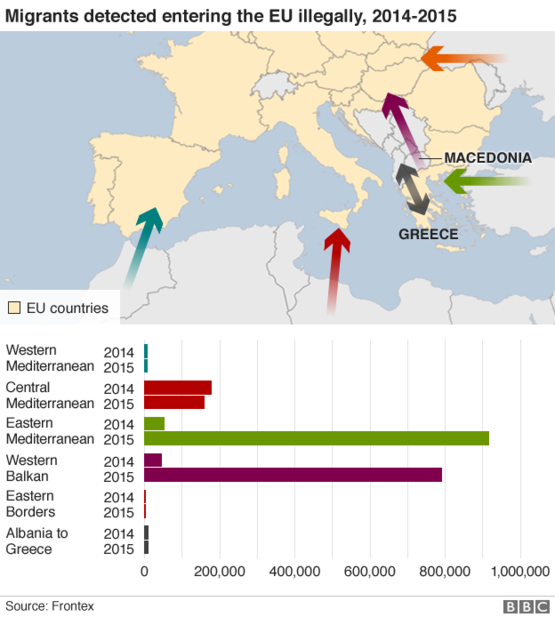
\includegraphics[width=0.8\linewidth]{images/routes_migrants}
		\caption{Routes towards EU used by refugees}
	\end{center}
\end{figure}

\newpage
Other migrants continue to travel by boat from Libya to Italy, a longer and more hazardous journey. 

Survivors often report violence and abuse by people traffickers, who charge thousands of dollars per person for their services. The chaos in Libya in particular has given traffickers freedom to exploit migrants and refugees desperate to reach Europe.

\subsection{What is their goal?}
Many attempting to reach Germany and other northern EU countries go via the perilous Western Balkans route, running the gauntlet of brutal people traffickers and robbers.

Faced with a huge influx of people, Hungary was the first to try to block their route with a razor-wire fence. The 175km (110-mile) barrier was widely condemned when it went up along the Serbia border, but other countries such as Slovenia and Bulgaria have erected similar obstacles.

Austria has placed a cap on the number of people allowed into its borders. And several Balkan countries, including Macedonia, have also decided only to allow Syrian and Iraqi migrants across their frontiers.

As a result, thousands of migrants have been stranded in makeshift camps in cash-strapped Greece, which has asked the European Commission for nearly €500m in humanitarian aid. 

\begin{figure}[!h]
	\begin{center}
		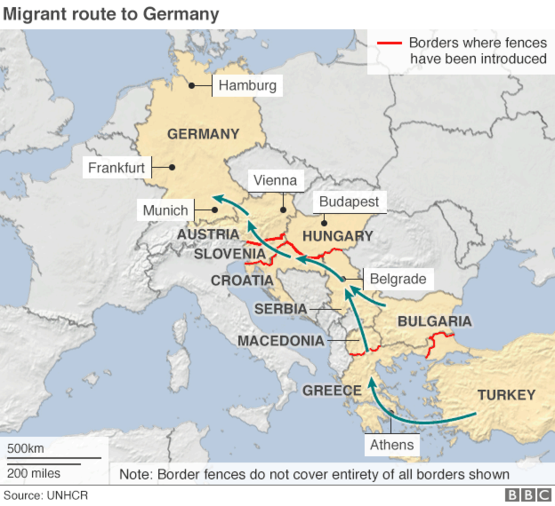
\includegraphics[width=0.7\linewidth]{images/journey_to_germany}
		\caption{Refugee route towards Germany}
	\end{center}
\end{figure}

Under an EU rule known as the Dublin regulation, refugees are required to claim asylum in the member state in which they first arrive.

But some EU countries, such as Greece, Italy, and Croatia, have been allowing people to pass through - often via the passport-free Schengen zone - to countries further north. And those countries are often failing to send migrants back.

Germany received more than 1.1 million asylum seekers 2015 - by far the highest number in the EU.

Hundreds of thousands of people are somewhere along the route, in Hungary, Croatia, Austria, Serbia, and elsewhere.

Meanwhile between 2,000 and 5,000 migrants are camped at the French port of Calais in the hope of crossing over to the UK.

\subsection{Fair share over EU countries?}

Germany has been critical of other EU countries - including France and the UK -over their relatively meagre commitments to take people in.

In September, EU interior ministers approved a controversial plan to relocate 120,000 migrants across the continent over the next two years, with binding quotas. Romania, the Czech Republic, Slovakia and Hungary opposed the scheme.

Despite some efforts to ease the burden on Italy and Greece, only small groups of migrants have been relocated so far and several states in Central and Eastern Europe have refused to accept them.

For years the EU has been struggling to harmonise asylum policy. That is difficult with 28 member states, each with their own police force and judiciary.

Championing the rights of poor migrants is difficult as the economic climate is still gloomy, many Europeans are unemployed and wary of foreign workers, and EU countries are divided over how to share the refugee burden.

\textbf{So summed up following facts clearly point out:}
\begin{itemize}
	\item largest refugee crisis since centuries
	\item dangerous way towards Europe
	\item Dublin regulation
	\item EU still struggling
	\item worse tragedies
		\subitem Austria, 71 dead Syrian refugees
	
\end{itemize}

\newpage
\section{Conclusion}

According to information gathered in 2013, there are 232 million of migrants. Migrant waves are mostly heading towards USA, Russia and Europe. These are mainly economic migrants. Others are forced migrants or refugees affected by wars or deconstruction of countries due to export of democracy and search for vast oil fields in the Middle East and all over the world. Refugee crisis in Europe encompasses economic, forced, illegal migrants and refugees. It is a heterogenous group on the move or a new Migration Period in the age of the second modernity. They are being currently used as a powerful biopolitical and potential economic weapon in conquering space and transforming cultural identities in the long run, as it is the case in Europe. Europe is being confronted with an unexpected refugee crisis. The case of refugee crisis, which exemplifies and shows the ugly side of globalization, has made Europe look like a bad tempered instrument of imaginary power in evident postmodern condition.
Multinational corporations are accused of social injustice, unfair working conditions, as well as lack of concern for environment, mismanagement of natural resources, and ecological damage. This causes many people to leave and find better places to live, like mentioned before.


